\documentclass[12pt]{article}
\usepackage[a4paper, total={6.5in, 8in}]{geometry}
\usepackage[english]{babel}
\usepackage{graphicx}
\usepackage[autostyle, english = american]{csquotes}
\MakeOuterQuote{"}
\usepackage{xargs}
\usepackage{longtable}
\usepackage{amsmath,amssymb}
\usepackage{tabularx}
\usepackage{hyperref}
\usepackage[dvipsnames]{xcolor}
\hypersetup{
    colorlinks=true,
    linkcolor=black,
    filecolor=magenta,      
    urlcolor=cyan,
    pdftitle={Overleaf Example},
    pdfpagemode=FullScreen,
    }

\newcolumntype{R}[1]{>{\raggedleft\arraybackslash}p{#1}}
\newcolumntype{L}[1]{>{\raggedright\arraybackslash}p{#1}}
%\newcolumntype{L}[1]{>{\raggedright\let\newline\\\arraybackslash\hspace{0pt}}p{#1}}

\newcounter{mycounter}
\newcommand{\rowlabel}[1]{\refstepcounter{mycounter} \label{#1}}

\begin{document}

	\title{\Huge Rulebook\\\large Battle of Causality}
	\author{Michal Horanský}
	\maketitle
	
	\tableofcontents
	
	\section{Introduction}
	\textit{Battle of Causality} is a turn-based digital strategy board game about time-travel. To address the elephant in the room which typically barges in at this point and loudly asks: "So how is it different from \textit{5D Chess With Multiverse Time Travel}?" In \textit{5D Chess With Multiverse Time Travel}, you cannot "change the past" in a way that affects a board configuration which has already been reached--attempting to do so creates a new timeline, which is a neat resolution of the ontological paradox. \textit{Battle of Causality} tackles time-travel in a completely different way, utilising the Novikov self-consistency principle. A stone may travel back in time, but such an action only occurs if it can be "justified" by the player's actions, i.e. any caused effects don't contradict their initial causes. In short, there is a single timeline which hosts an increasing number of tangled world lines, where effect may precede cause, and the growing danger of a paradox looms ever-present.
	
	\subsection{Setting}
	\begin{quote}
	\textit{Cover blown, those few souls made their mad dash towards the enemy's fragile heart, trapped impossibly between the rattle of weaponry and the clock rapidly bleeding time. Yet, in the eleventh hour, they found the rivers of blood running upstream, they witnessed the intangible skein wound from all their struggle undoing itself, until all this impossible movement dissolved into anticipation. Now they face the same odds, and the same struggle, but the scales have been tipped. Now it is they who observe and are not observed, until the moment arises when they tap the shoulder of the man turning his back to face them. Seeing pictures from their pasts running past, object and image converge and the mirror breaks again and again. We found in that point of eternal return the very source of struggle itself: anticipation.}
	\end{quote}
	Two players, $A$ and $B$, face each other in a competitive battle over the board. Each player controls an army of stones with diverse specialisations and abilities. Commandeering their stones as time progresses, the players attempt to destroy the opponent's army to clear the way for capturing all the strategically significant points. However, time runs short, and after a few turns, there is nowehere to move anymore. The game, however, continues: the stones can be commanded not just to move in space, but also to jump back in time. These new versions of the old stones share the board space with their previous versions, which follow the established routes already known to the players. However, should a stone travel back in time and obstruct the path of its old self, history becomes malleable. And so the players can control an ever-growing and ever-changing army of many mirror images of a handful of stones, which constantly rewrite their own history. However, be careful not to perform an action which contradicts itself, or you might find yourself trapped in a paradox...
	
	\subsection{Goal of the game}
	
	The board houses a few special squares called bases. Each base has an allegiance: It can belong to either player, or be neutral. Players can capture bases by visiting them with their stones, which changes the base's allegiance to the player's faction until it is captured by their opponent. The goal of the game is to make sure that all the bases on the board belong to you.
	
	\section{How to play}
	The board consists of squares placed along three axes: horizontal position $x$, vertical position $y$, and time $t$. Time is, of course, special, as the state of the squares at a particular time is directly inferred from the state of the squares at a lower time. The collection of squares at a specified time is called a time-slice, and can be thought of as the temporal equivalent of a rank or a file in classical chess. The dimension of the board along the time axis is called the time cap: the whole game takes place in a time interval of length restricted by this time cap.
	
	\begin{figure}[h]
\begin{center}

    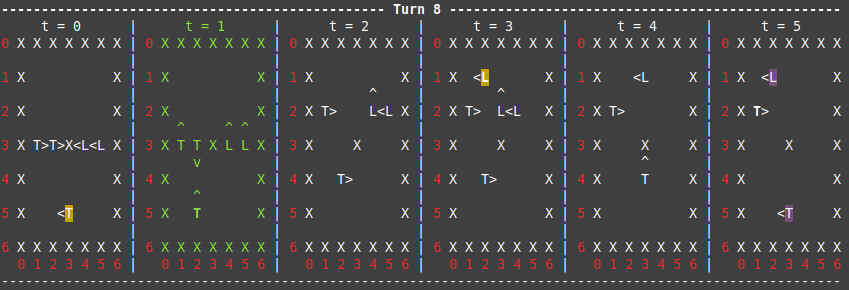
\includegraphics[width=0.9\textwidth]{images/diag_game_example}
 \caption{This is an example of a game in-progress. This board has a time cap of $6$, so there are six time-slices organized from earliest to latest, left to right. Player $A$ and player $B$'s stones are labelled T and L, respectively. The game is already on turn $8$, which for this time cap corresponds to round $2$ and active time-slice $t=1$. In the active time-slice, player $A$ has only one causally free stone at $(x=2, y=5)$ which they can command in this turn, and player $B$ will not be able to place down any flags until turn $10$, where they have a causally free stone at $(x=2, y=1)$.}\label{fig:placing flags}
\end{center}
\end{figure}
	
	The game is played in rounds, where every round consists of a number of turns equal to the time cap. In each round, the players look at the first time-slice in the first turn, then the second time-slice in the second turn etc, until they reach the time cap. In each turn, both players simultaneously place down flags in the active time-slice, which are essentially commands for their stones, and after each turn, those flags are translated into actions performed by the stones, which determine the state of the next time-slice.
	
	At the end of each round, a procedure called \textbf{canonisation} is performed, which resolves everything to do with time-travel and sets the stage for the first time-slice of the next round. At this moment, it is also checked if the end-of-game conditions have been satisfied.
	
	An important thing to note is that a flag being placed for a stone at a time-slice $t$ affects the stone "in-between" this and the next time-slice, and the consequences of that action showly on in the next time-slice $t+1$.
	
	\subsection{Stone trajectories and flag placement}
	Every stone placed on the board has a unique flag called the \textbf{progenitor} which, if active, places it onto a specific position. From the corresponding time onwards, the stone checks the square it stands on in each time-slice for flags which can be activated (see Sec. \ref{sec:flag activation conditions}). Activating a flag determines the stone's initial placement in the next time-slice, and after all flags in this time-slice are dealt with, this initial placement is changed into the canonical placement by resolving all conflicts (see Sec. \ref{sec:spatial conflict resolution}). If the stone follows a flag which removes it from a board, is destroyed, or becomes causally free, it is not placed into the next time-slice, and its trajectory ends.
	
	\begin{figure}[h]
\begin{center}

    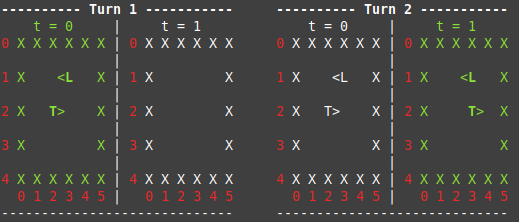
\includegraphics[width=0.6\textwidth]{images/diag_placing_flags}
 \caption{This is a board with a time cap of $2$. In the first turn of the round, two stones are placed on setup, but since they are causally free (see Sec. \ref{sec:causal freedom}), they are not present in time-slice $t=1$. In the first turn, player $A$ tells their tank to move forward by one square, and player $B$ tells their tank to wait. Hence, in second turn, the two stones are placed in both time-slices, being causally free only in time-slice $t=1$.}\label{fig:placing flags}
\end{center}
\end{figure}
	
	\subsubsection{Causal freedom}\label{sec:causal freedom}
	If a stone reaches a position at which there is no flag which it can follow, the stone becomes \textbf{causally free}. This means that we don't know what the stone does between this and the next time-slice, and so it isn't yet placed in the next time-slice. However, when a flag is placed for this stone at the point of its causal freedom, it gets "locked" into the specified action and can be placed into the next time-slice, where (if not destroyed) it is causally free and can be commanded again.
	
	Now we understand the structure of the game as divided into rounds and turns: the turns progress through every time-slice "sweeping up" causally free stones, propagating their trajectories to the point of removal from the board or the time cap. Then, when the end of the round is reached, any progenitor flag, including the newly placed time-jumps, can be set as active, which in turn creates new causally free stones sprinkled over the board, and a new round of "sweeping" may begin again.
	
	\subsubsection{Preventing amnesia}\label{sec:flag activation conditions}
	Firstly, a flag (which is not a progenitor) associated with a stone requires that stone to be present at its position in order to be activated. However, this is a necessary, but not a sufficient condition. Consider the situation outlined in Fig. \ref{fig:amnesia}.
	
\begin{figure}[h]
\begin{center}
    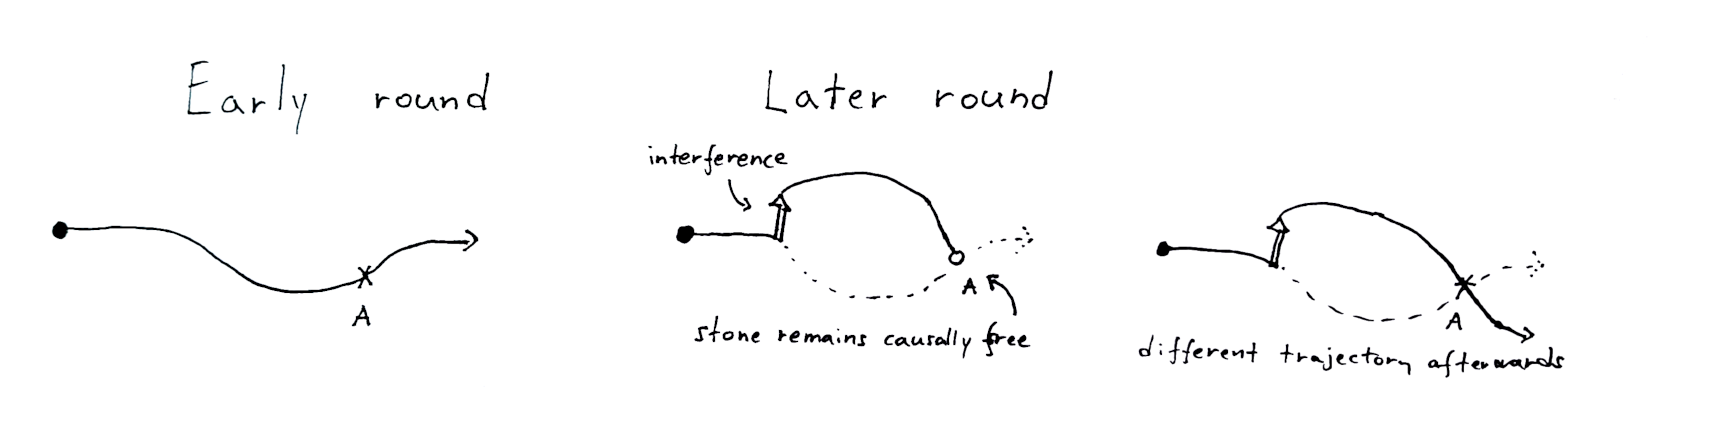
\includegraphics[width=1\textwidth]{images/diag_amnesia}
 \caption{A stone follows a certain trajectory in an early round, where it reaches position $A$ and an associated flag is placed for it at that position. In a later round, the stone's trajectory is broken by interference preceding $A$, and the stone takes a different trajectory. However, the new trajectory also reaches point $A$. Now: at $A$, a flag already exists for this stone in this later round. Nevertheless, this flag does \textit{not} get activated, because it was placed in an earlier round than the flags the stone already followed along this later trajectory. The stone doesn't "forget" the interference, and it doesn't slip into an old trajectory if given the chance. The trajectory from the earlier round may still get realised in an even later round if the interference effect disappears from the canon.}\label{fig:amnesia}
\end{center}
\end{figure}
	
	
	Therefore, the general rule is as follows: If multiple active flags associated with a stone at a specific position exist at that position, the flag placed in the \textit{earliest round which is not earlier than the last flag the stone followed in the previous time-slice} is activated.
	
	\subsubsection{Order of flag execution}
	
	something something the order to obtain the canonical state of a time-slice $t$:
	\begin{enumerate}
		\item The movement flags placed on the previous time-slice and progenitor flags associated with this time-slice are executed, propagating the stones into this time-slice, in general into conflicting positions.
		\item The spatial conflicts are resolved.
		\item The stone actions activated in the previous time-slice, such as attacks, and board events such as the explosion of bombs and tagscreens, are resolved now. Since these can only remove stones from the board, but not push them, the time-slice remains without conflict.
		\item Finally, the allegiance of each base changes to the faction of the occupying stone, if there is one. The time-slice state is now canonical.
	\end{enumerate}
	
	\subsection{Spatial movement}
	The simplest action a stone typically performs is moving spatially.
	
	\subsubsection{Spatial conflict resolution}\label{sec:spatial conflict resolution}
	
	\subsection{Interacting with the past}
	
	\subsubsection{Rule of dogma}\label{sec:rule of dogma}
	\begin{quote}
	All ante-effects placed in this round are dogmatic in the next round.
	\end{quote}
	
	\subsubsection{Jumping back in time} \label{sec:timejumps}
	
	\subsubsection{Other interactions with the past}
	
	
	\section{Stone types}\label{sec:stone types}
	There are multiple types of stones, a multitude of which may be at each player's disposal throughout the game. These stones differ in their ways of moving, attacking, time-jumping etc. The following is a list of the stone types currently in the game\footnote{The game is open-source, and I encourage you all to add all the new stone types you can think of!}:
	\begin{itemize}
	\item \textbf{Tank}
		\begin{itemize}
		\item Opposable
		\item Orientable
		\item Movement: the tank can move forwards or backwards by 1 square and then optionally turn clockwise or anticlockwise by a quarter-revolution. Alternatively, it can stay on its square and turn to any azimuth, or remain as it is.
		\item Attacking: the tank attacks by firing in the direction of its azimuth, destroying the first stone in its line of sight, regardless of the stone's faction.
		\item Time-jumps: the tank can only time-jump after reaching the final time-slice.
		\end{itemize}
	\item \textbf{Bombardier}
		\begin{itemize}
		\item Opposable
		\item Unorientable
		\item Movement: the bombardier can move by $1$ square in each of the $4$ cardinal directions.
		\item Attacking: the bombardier attacks by dropping a bomb onto the same spatial position in any previous time-slice. Being an ante-effect, the consequences of the attack don't unfold until the next round. The bomb destroys any stone on the target square and all of the $4$ adjanced squares.
		\item Time-jumps: the bombardier can only time-jump after reaching the final time-slice.
		\end{itemize}
	\item \textbf{Sniper}
		\begin{itemize}
		\item Opposable
		\item Orientable
		\item Movement: the sniper cannot move on its own, and relies on being pushed by other opposable stones. However, it can turn to any azimuth or remain as it is.
		\item Attacking: the sniper attacks by firing in the direction of its azimuth, destroying the first stone in its line of sight except for stones in the same faction. Stones in the same faction are ignored and the attack can hit even stones obscured behind them.
		\item Time-jumps: the sniper can time-jump from any time-slice into any previous time-slice.
		\end{itemize}
	\item \textbf{Tagger}
		\begin{itemize}
		\item Unopposable
		\item Unorientable
		\item Movement: the tagger jumps like a horse (two squares in any cardinal direction and one square in a perpendicular direction). Being unopposable, it naturally jumps over other stones.
		\item Attacking: the tagger deploys a tagscreen at its position, which explodes one turn later, tagging any stone on its square and all of the $4$ adjanced squares. The tagged stones lose their ability to time-jump and become causally locked in the final time-slice.
		\item Time-jumps: the tagger can time-jump at any time, but its time-jumps still obey the rules of its movement--either by two time-slices back and by one square in any cardinal direction, or by one time-slice back and by two squares in any cardinal direction.
		\end{itemize}
	\item \textbf{Wildcard}
		\begin{itemize}
		\item Unopposable
		\item Unorientable
		\item Movement: the wildcard jumps onto the neighbouring square in any of the $4$ cardinal or $4$ diagonal directions.
		\item Attacking: the wildcard can attack any single square in any of the $4$ cardinal or $4$ diagonal directions. Its attacks, if misdirected, will destroy even a stone of the same faction.
		\item Time-jumps: the wildcard can time-jump at any time. A special property of the wildcard is that it can swap the time-jump of any stone type (and is not limited by the azimuth if changing into an orientable stone). For more details on swapping, see Sec. \ref{sec:timejumps}.
		\item The wildcard cannot capture bases.
		\end{itemize}
	\end{itemize}
	
	\section{Ruleset variations}
	
	\section{Asymmetry and rating}
	The game may be, but is not necessarily symmetric for the players.
	
	\section{Glossary}
{\renewcommand{\arraystretch}{0.5}
 \begin{longtable}{ R{0.15\linewidth}  L{0.81\linewidth}  }

\rowlabel{glossary:active} \\* \textbf{active} & \parbox[t]{\linewidth}{This term may depend mulitple things depending on the context. A flag is said to be active if its activity has been set as such in a scenario. A time-slice is said to be active in every turn in which the players are prompted to command their stones in that time-slice. See \hyperref[glossary:activity]{\textbf{activity}}, \hyperref[glossary:turn]{\textbf{turn}}.}\\
\rowlabel{glossary:activity} \\* \textbf{activity} & \parbox[t]{\linewidth}{A flag can be set as active or passive. An active flag behaves normally. A passive flag is ignored by the stone it's attached to, and the stone behaves as if the flag was not placed at all. See \hyperref[glossary:flag]{\textbf{flag}}, \hyperref[glossary:active]{\textbf{active}}.}\\
\rowlabel{glossary:allegiance} \\* \textbf{allegiance} & \parbox[t]{\linewidth}{A property of a base, determining the last faction which conquered that base, or "neutral" if determined as such on setup. See \hyperref[glossary:faction]{\textbf{faction}}.}\\
\rowlabel{glossary:ante-effect} \\* \textbf{ante-effect} & \parbox[t]{\linewidth}{An effect that precedes its cause on the time-axis. See \hyperref[glossary:retro-cause]{\textbf{retro-cause}}.}\\
\rowlabel{glossary:azimuth} \\* \textbf{azimuth} & \parbox[t]{\linewidth}{The orientation of an orientable stone, which can be up (negative $y$ direction), right (positive $x$ direction), down (positive $y$ direction), or left (negative $x$ direction). See \hyperref[glossary:orientable]{\textbf{orientable}}.}\\
\rowlabel{glossary:base} \\* \textbf{base} & \parbox[t]{\linewidth}{A square which can be captured by a player visiting it with one of their stones, and it remains captured until their opponent visits it themselves. The goal of the game is to reach a scenario where all the bases end up captured by your stones in the final time-slice. See \hyperref[glossary:allegiance]{\textbf{allegiance}}.}\\
\rowlabel{glossary:canon} \\* \textbf{canon} & \parbox[t]{\linewidth}{The canon of the board is its evolution throughout the turns of the game. Even though time may go back, turns always progress forward, and once the state of the board for a specific turn has been determined, it cannot change again--we say it is canonical. A canonical state cannot be conflicting. See \hyperref[glossary:conflicting]{\textbf{conflicting}}.}\\
\rowlabel{glossary:canonisation} \\* \textbf{canonisation} & \parbox[t]{\linewidth}{At the end of each round, the highest-priority causally consistent scenario is selected for the next round based on the flags placed so far, omitting ante-effects placed in the round which just ended. See \hyperref[glossary:causally consistent]{\textbf{causally consistent}}.}\\
\rowlabel{glossary:causally consistent} \\* \textbf{causally consistent} & \parbox[t]{\linewidth}{Not resulting in a paradox. See \hyperref[glossary:scenario]{\textbf{scenario}}, \hyperref[glossary:paradox]{\textbf{paradox}}.}\\
\rowlabel{glossary:causally free} \\* \textbf{causally free} & \parbox[t]{\linewidth}{A stone is causally free at a specific position if it is placed on the board at that position, but is not subject to a flag at that position.}\\
\rowlabel{glossary:causally locked} \\* \textbf{causally locked} & \parbox[t]{\linewidth}{Present on the board, but not causally free. See \hyperref[glossary:causally free]{\textbf{causally free}}.}\\
\rowlabel{glossary:comb rule} \\* \textbf{comb rule} & \parbox[t]{\linewidth}{The comb rule states that for each turn there may be no causally free stones in time-slices preceding the active time-slice. Therefore, for all but the final time-slice each player must command all of their causally free stones.}\\
\rowlabel{glossary:conflicting} \\* \textbf{conflicting} & \parbox[t]{\linewidth}{Not adhering to the rules which specify what the board can and cannot look like. Typically, the movement of stones in each turn sends them into conflicting positions, which are subsequently resolved by the game to find the canonical state of the next time-slice. See \hyperref[glossary:canon]{\textbf{canon}}.}\\
\rowlabel{glossary:dogma} \\* \textbf{dogma} & \parbox[t]{\linewidth}{A flag is said to be dogmatic in a specific round if it is set as active in the round's scenario due to a special rule (the \hyperref[sec:rule of dogma]{rule of dogma}), not because it was set as active due to the selection of a high-priority causally consistent scenario. See \hyperref[glossary:rule of dogma]{\textbf{rule of dogma}}.}\\
\rowlabel{glossary:faction} \\* \textbf{faction} & \parbox[t]{\linewidth}{A player; i.e. "this stone's faction" synonymous to "the player this stone belongs to".}\\
\rowlabel{glossary:flag} \\* \textbf{flag} & \parbox[t]{\linewidth}{A command placed at a specific position, for a specific stone, by the player. Flags can order the stones to attack, move, time-jump etc.}\\
\rowlabel{glossary:interference} \\* \textbf{interference} & \parbox[t]{\linewidth}{The act of obstructing the trajectory of a stone established in previous rounds. This makes the stone causally free again, but can also prevent it from activating its associated retro-causes.}\\
\rowlabel{glossary:opposable} \\* \textbf{opposable} & \parbox[t]{\linewidth}{If a stone is opposable, then it moves in a way which allows it to push other stones, but its movement can also be blocked by a stone moving in the opposite direction. See \hyperref[glossary:unopposable]{\textbf{unopposable}}.}\\
\rowlabel{glossary:orientable} \\* \textbf{orientable} & \parbox[t]{\linewidth}{If a stone is orientable, then its trajectory is described not only by its positions, but also their corresponding azimuths. Orientable stones move and attack in ways which depend on their azimuth. See \hyperref[glossary:azimuth]{\textbf{azimuth}}.}\\
\rowlabel{glossary:paradox} \\* \textbf{paradox} & \parbox[t]{\linewidth}{A scenario such that if we evolve the board along the time axis, there will either be active ante-effects which have zero or multiple activated retro-causes, or activated retro-causes which correspond to an inactive ante-effect.}\\
\rowlabel{glossary:position} \\* \textbf{position} & \parbox[t]{\linewidth}{One square on the board in one specific time-slice. Parametrised by three numbers: (t, x, y). See \hyperref[glossary:spatial position]{\textbf{spatial position}}, \hyperref[glossary:causally free]{\textbf{causally free}}.}\\
\rowlabel{glossary:precede} \\* \textbf{precede} & \parbox[t]{\linewidth}{Occur in a time-slice with time smaller than}\\
\rowlabel{glossary:priority} \\* \textbf{priority} & \parbox[t]{\linewidth}{Every scenario has a priority. If two or more scenarios are causally consistent for a round, the one with highest priority is canonised. See \hyperref[glossary:scenario]{\textbf{scenario}}, \hyperref[glossary:canonisation]{\textbf{canonisation}}.}\\
\rowlabel{glossary:progenitor} \\* \textbf{progenitor} & \parbox[t]{\linewidth}{A progenitor is a flag which, when active, places a new stone onto its associated position. Progenitors are unique in the way that they are associated with a specific stone, but do not require the presence of that stone at their position to be activated--rather, when activated, they place the stone themselves.}\\
\rowlabel{glossary:recency} \\* \textbf{recency} & \parbox[t]{\linewidth}{A property of ante-effects and stones, determined depending on the specific ruleset (see Sec. \ref{sec:ruleset variations}). Stones and ante-effects with higher recency are more likely to be preserved during canonisation if two or more causally consistent scenarios are possible.}\\
\rowlabel{glossary:retro-cause} \\* \textbf{retro-cause} & \parbox[t]{\linewidth}{A cause that occurs after its effect on the time-axis. We say that a retro-cause is \textit{activated} if it is executed by its corresponding stone at its position in some specific scenario. See \hyperref[glossary:ante-effect]{\textbf{ante-effect}}.}\\
\rowlabel{glossary:round} \\* \textbf{round} & \parbox[t]{\linewidth}{The progress of the game occurs in rounds. In each round, players command their stones for every time-slice with increasing time, and after reaching the end, the round is canonised. See \hyperref[glossary:turn]{\textbf{turn}}, \hyperref[glossary:canonisation]{\textbf{canonisation}}.}\\
\rowlabel{glossary:rule of dogma} \\* \textbf{rule of dogma} & \parbox[t]{\linewidth}{All ante-effects placed in this round are dogmatic in the next round. See \hyperref[glossary:dogma]{\textbf{dogma}}.}\\
\rowlabel{glossary:scenario} \\* \textbf{scenario} & \parbox[t]{\linewidth}{A scenario for a given round specifies which ante-effects placed in all the previous rounds are active and which are passive in that round, and which setup placements are omitted. See \hyperref[glossary:activity]{\textbf{activity}}, \hyperref[glossary:setup]{\textbf{setup}}.}\\
\rowlabel{glossary:setup} \\* \textbf{setup} & \parbox[t]{\linewidth}{A set of progenitors which place stones on the board in the first time-slice. See \hyperref[glossary:progenitor]{\textbf{progenitor}}.}\\
\rowlabel{glossary:spatial position} \\* \textbf{spatial position} & \parbox[t]{\linewidth}{One square on the board across all time-slices. Parametrised by two numbers: (x, y). See \hyperref[glossary:position]{\textbf{position}}.}\\
\rowlabel{glossary:stone} \\* \textbf{stone} & \parbox[t]{\linewidth}{A stone is a unit which belongs to a player and is commanded by them, or is neutral (for example a box or a mine). The term \textbf{stone} implies continuity across time-slices but not across time-jumps. In other words, if a stone is placed on the board in the first time-slice and then makes a series of spatial moves, which propagate it into the final time-slice, we say it is still the same stone; however, if that stone then jumps back in time into the first time-slice, we say that the stone placed in the first time-slice is another, new stone. See \hyperref[glossary:worldline]{\textbf{worldline}}.}\\
\rowlabel{glossary:swap} \\* \textbf{swap} & \parbox[t]{\linewidth}{To swap an ante-effect means to add a new retro-cause to it, which can prevent its deactivation during subsequent canonisations, but can also result in a paradox if the number of retro-causes becomes too big. See \hyperref[glossary:paradox]{\textbf{paradox}}.}\\
\rowlabel{glossary:time} \\* \textbf{time} & \parbox[t]{\linewidth}{An axis on the board, akin to horizontal and vertical position.}\\
\rowlabel{glossary:time cap} \\* \textbf{time cap} & \parbox[t]{\linewidth}{The length of the time axis. The value of time runs from $0$ to $(\text{time cap}) - 1$.}\\
\rowlabel{glossary:time-jump} \\* \textbf{time-jump} & \parbox[t]{\linewidth}{The act of jumping back in time. For every stone, there will be opportunity to make a time-jump and re-join the game in the next round, when the earlier time-slices become available to place flags in once again.}\\
\rowlabel{glossary:time-slice} \\* \textbf{time-slice} & \parbox[t]{\linewidth}{A section of the board specified by a given value of time. Analogous to "rank" and "file" for horizontal and vertical position in chess.}\\
\rowlabel{glossary:trajectory} \\* \textbf{trajectory} & \parbox[t]{\linewidth}{The set of positions along the time axis of a stone from the time when it was placed on the board until the time it was removed from the board, or became causally free.}\\
\rowlabel{glossary:turn} \\* \textbf{turn} & \parbox[t]{\linewidth}{Every round is divided into a number of turns equal to the time cap. Each turn corresponds to one time-slice (the \textbf{active} time-slice), and in each turn every player places down flags for their causally free stones in that time-slice. See \hyperref[glossary:round]{\textbf{round}}, \hyperref[glossary:active]{\textbf{active}}.}\\
\rowlabel{glossary:unopposable} \\* \textbf{unopposable} & \parbox[t]{\linewidth}{If a stone is unopposable, then it essentially jumps over other stones, and thus cannot be blocked by a stone moving in the opposite direction. However, such a stone's movement is always blocked when it attempts to jump onto an occupied square, since it is unable to push other stones. See \hyperref[glossary:opposable]{\textbf{opposable}}.}\\
\rowlabel{glossary:unorientable} \\* \textbf{unorientable} & \parbox[t]{\linewidth}{If a stone is unorientable, then its trajectory is described only by its positions. The movement and attack pattern of unorientable stones is symmetric under rotation by a quarter-revolution. See \hyperref[glossary:orientable]{\textbf{orientable}}.}\\
\rowlabel{glossary:worldline} \\* \textbf{worldline} & \parbox[t]{\linewidth}{A worldline is a collection of trajectories belonging to a sequence of stones where each stone ends their trajectory by a time-jump which creates the next stone. A worldline can change its structure as the game progresses, by interference and swapping. See \hyperref[glossary:trajectory]{\textbf{trajectory}}, \hyperref[glossary:swap]{\textbf{swap}}.}


\end{longtable}}
	
	
	
	
	
	

	
	
\end{document}
